%----------------------------------------------------------------------------------------------
%------ POSL
%----------------------------------------------------------------------------------------------
\chapter{A Parallel-Oriented Language for Modeling Constraint-Based Solvers}
\label{chap:posl}
\textit{In this chapter we introduce \posl{} as our main contribution and a new way to solve \csps{}. We resume its characteristics and advantages, and we get into details in the next sections. We describe a general outline to follow in order to build parallel solvers using \posl, and following each step is described in details.}
\vfill
\minitoc
\newpage

In this chapter we present the different steps to follow to build communicating parallel solvers with \posl. 
First of all, the algorithm that we have conceived to solve the target problem is modeled by decomposing it into small modules of computation. After that, they are implemented as separated {\it functions}. We name them \oms{} (see Figure~\ref{subfig:modules}, blue shapes). The coder's experience is crucial to find a good decomposition of its algorithm, because it will have an important impact in its future reuse and variability. The next step is to decide what information is interesting to receive from other solvers. This information is encapsulated into another kind of component called \opch, allowing data transmission among solvers (see Figure~\ref{subfig:modules}, red shapes).
In a third stage, is to glue the modules through \posl{}'s inner language (the reader can see an example in Appendix \tet{[...]}) to create independent solvers.
The parallel-oriented language based on operators that \posl{} provides (see Figure~\ref{subfig:as}, green shapes) allows not only the information exchange, but also executing components in parallel. In this stage, the information that is interesting to share with other solvers, is sent using operators. After that, we can connect them using {\it communication operators}. We call this final entity a {\it solvers set} (see Figure~\ref{subfig:conn}).

\begin{figure}[h]
	\centering
	\subfloat[][Creating \posl's modules]{
		\label{subfig:modules}
		
\includegraphics[width=0.4\linewidth]{modules.png}
	}\\
	\subfloat[][Assembling modules using \posl's operators]{%
		\label{subfig:as}
		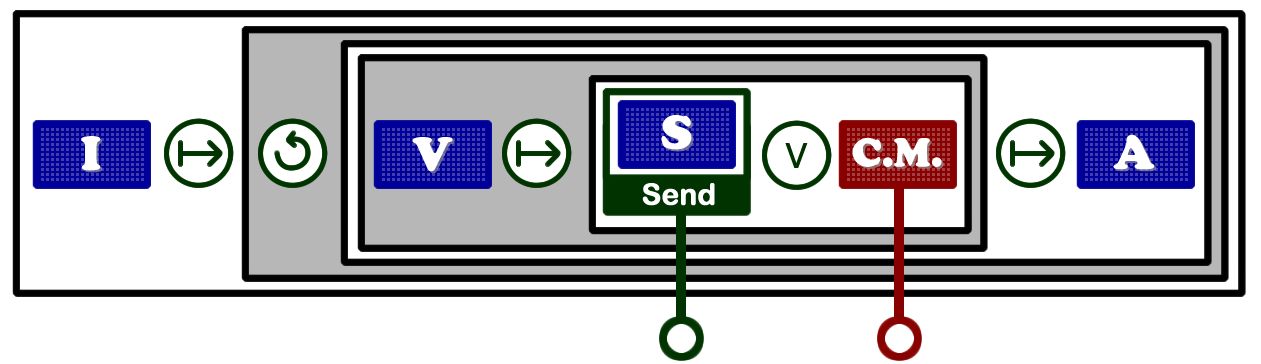
\includegraphics[width=0.6\linewidth]{as.png}
	}\\
	\subfloat[][Connecting \posl{} solvers to create \comstrs]{%
		\label{subfig:conn}
		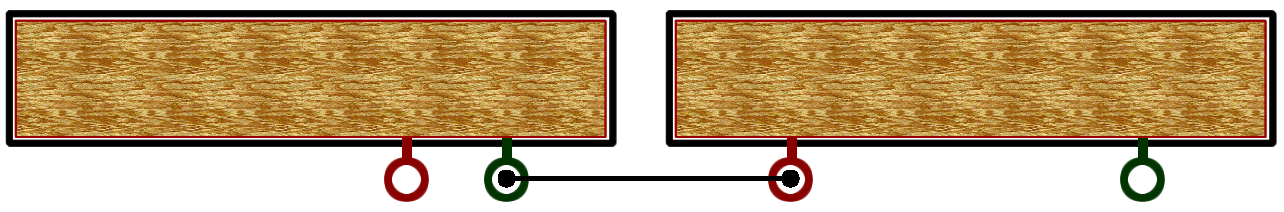
\includegraphics[width=0.6\linewidth]{conn.png}
	}
	\caption[]{Solver construction process using \posl}
	\label{fig:posl}
\end{figure}

Once the solvers set is ready, the last step is to model the problem to solve. To do so, the user must follow the framework specification to implement the benchmark, respecting some requirements. The most important one is to implement a {\it cost function} computing the cost for a given configuration, i.e., an integer indicating how much the configuration violates the set of constraints. This integer equals zero if the configuration is a solution.

\section{First Stage: Creating \posl's modules}

There exist two types of basic modules in \posl: \oms{} and \opchs{}. A \om{} is a function receiving an input, then executes an internal algorithm, and returns an output. A \opch{} is also a function receiving and returning information, but in contrast, the \opch{} can receive information from two different ways: through parameter or from outside, i.e. by communicating with a module from another solver.

\subsection{Computation Module}

%In this sub-section we expose the definition and the characteristics and the details of the \om, and give some examples. We explain how to create new \oms{} using the basic layer of the framework.

A \om{} is the most basic and abstract way to define a piece of computation. It is a function receiving an input, then executing an internal algorithm, and returning an output. The input and output types will characterize the computation module signature. It can be dy\-na\-mi\-cally replaced by or combined with other computation modules, since they can be shared among solvers working in parallel. They are joined through \ass.

\defname{Computation Module}{
A \om{} $Cm$ is a mapping defined by: 
\begin{equation}
\label{def:om}
Cm:D \rightarrow I
\end{equation}
}

$D$ and $I$ can be either a set of configurations, or set of sets of configurations, or a set of values of some data type, etc.

Consider a local search meta-heuristic solver. One of its \oms{} can be the function returning the set of configurations composing the neighborhood of a given configuration:

\begin{equation*}
Cm_{neighborhood}:D_1\times D_2\times\dots\times D_n \rightarrow 2^{D_1\times D_2\times\dots\times D_n}
\end{equation*}

\noindent where $D_i$ represents the definition domains of each variable of the input confi\-gura\-tion.

Figure~\ref{fig:om} shows an example of computation module: it receives a configuration $S$ and then computes the set $V$ of its neighbor configurations $\left\{S^1, S^2, \dots, S^m\right\}$.

\vspace{0.5cm}
\begin{figure}
	\centering	
	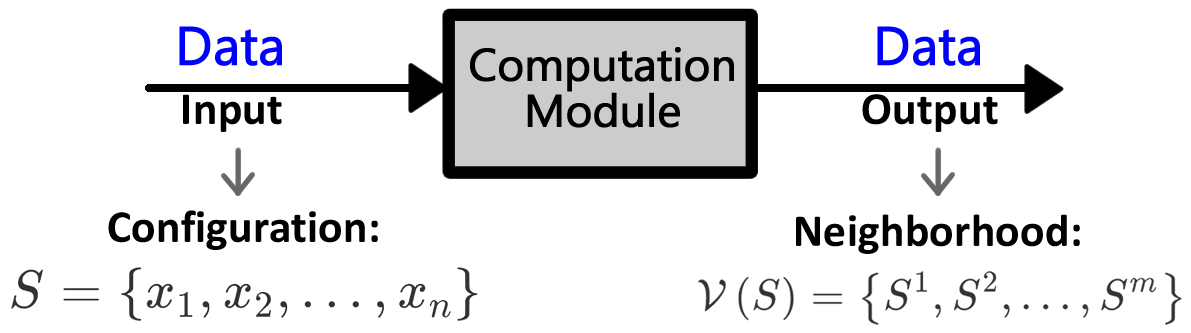
\includegraphics[width=0.7\linewidth]{OM.png}
	\caption{An example of a computation module computing a neighborhood}\label{fig:om}
\end{figure}

\subsection{Communication modules}

%In this sub-section we expose the definition and the characteristics and the details of the \opch, and give some examples. We explain how to create new \opchs{} using the basic layer of the framework.

A \opch{} is also a function receiving and returning its information, but in contrast, the \opch{} can receive information from two different ways: through input or from outside, i.e., by communicating with a module from another solver. A \opch{} is the component in charge of the information reception in the communication between solvers (we will talk about information transmission in the next section). They can interact with \oms{} through operators (see Figure~\ref{fig:och}).

A \opch{} can receive two types of information, always coming from an external solver: data or \oms{}. It is important to notice that when we are talking about sending/receiving \oms, we mean sending/receiving only required information to identify it and being able to instantiate it.

In order to distinguish from the two types of \opchs, we will call Data Communication Module the \opch{} responsible for the data reception (Figure~\ref{subfig:doch}), and Object Communication Module the one responsible for the reception and instantiation of \oms{} (Figure~\ref{subfig:ooch}).

\defname{Data Communication Module}{
A \emph{Data Communication Module} $Ch$ is a component that produces a mapping defined as follows: 
\begin{equation}
\label{def:dopench}
Ch:U \rightarrow I
\end{equation}
It returns the information $I$ coming from an external solver, no matter what the input $U$ is.
}

\defname{Object Communication Module}{
	If we denote by $\mathbb{M}$ the space of all the \oms{} defined by Definition \ref{def:om}, then an \emph{Object Communication Module} $Ch$ is a component that produces a \om{} coming from an external solver as follows:
	\begin{equation}
	\label{def:oopench}
	Ch:\mathbb{M} \rightarrow \mathbb{M}
	\end{equation}
}%

\begin{figure}
	\centering
	\subfloat[][Data \opch]{
		\label{subfig:doch}
		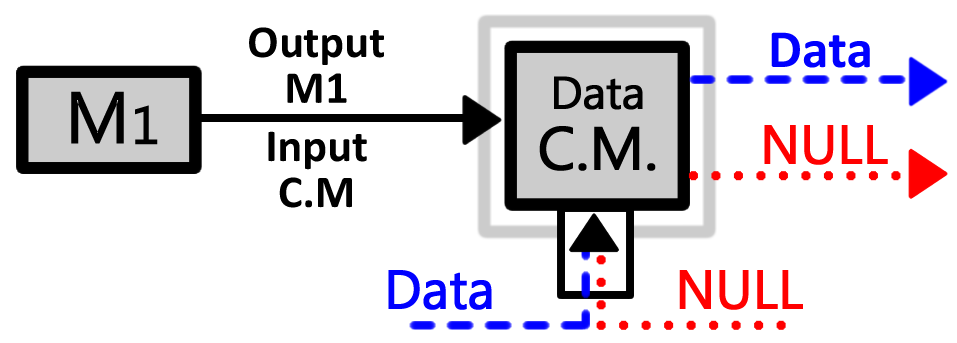
\includegraphics[width=0.4\linewidth]{D_OCh.png}
	}
	\hspace{0.05\textwidth}%
	\subfloat[][Object \opch]{%
		\label{subfig:ooch}
		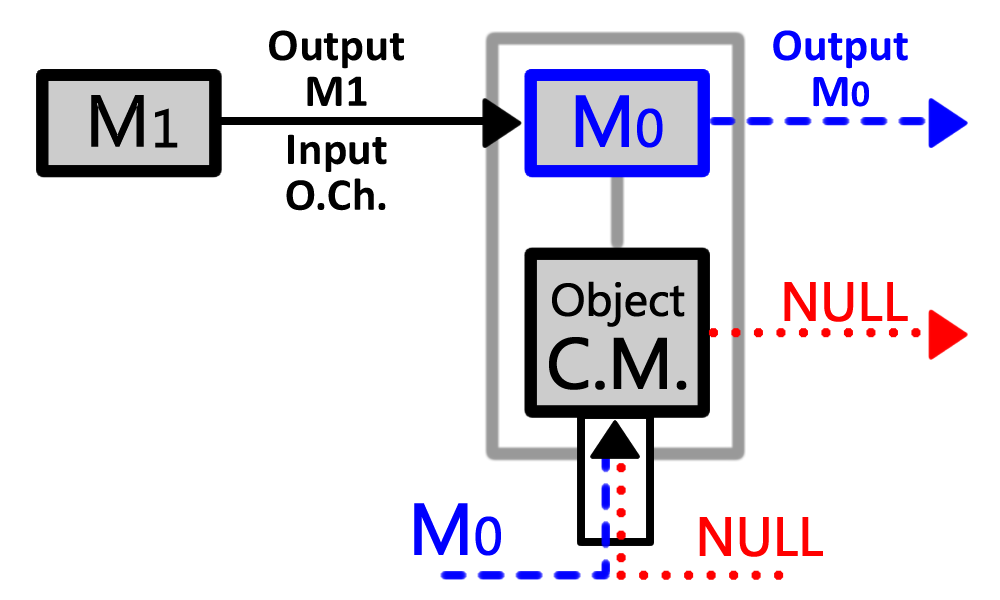
\includegraphics[width=0.4\linewidth]{O_OCh.png}
	}
	\caption[]{Communication module}
	\label{fig:och}
\end{figure}

Users can implement new computation and connection modules but \posl{} already contains many useful modules for solving a broad range of problems.

Due to the fact that \opchs{} receive information coming from outside and have no control on them, it is necessary to define the {\it NULL} information, to denote the absence of any information. If a Data Communication Module receives a piece of information, it is returned automatically. If a Object Communication Module receives a \om{}, the latter is instantiated and executed with the \opch's input, and its result is returned. In both cases, if no available information exists (no communications performed), the \opch{} returns the {\it NULL} object.

\section{Second Stage: Assembling \posl's modules}
\label{subsec:2ndstage}

Modules mentioned above are defined respecting the signature of some predefined abstract module. For example, the module showed in Figure~\ref{fig:om} is a \om{} based on an abstract module that receives a configuration and returns a neighborhood. In that sense, an example of a concrete \om{} (or just \om{} for simplification sake) can be a function receiving a configuration, and returns a neighborhood composed of $N$ configurations only differing from one value to the input configuration.

In this stage an \as{} is coded through \posl{}. It takes abstract modules as {\it parameters} and combines them with operators. Through the abstract solver, we can also decide what information to be sent to other solvers, by using some operators to send the result of a computation module (see below). Following we present a formal and more detailed presentation of \posl{}'s operators specification. 


The \as{} is the solver's backbone. It joins the \oms{} and the \opchs{} coherently. It is independent from the \oms{} and \opchs{} used in the solver. It means they can be changed or modified during the execution, without altering the general algorithm, but still respecting the main structure. \modified{Each time we combine some of them using \posl's operators, we are creating a \cm. Following we define formally the concept of \textit{module} and \cm.}

\begin{definition}
	\label{def:module}
We call {\bf module} to (and it is denoted by the letter $\mathcal{M}$):
\begin{enumerate}\renewcommand{\labelitemi}{\scriptsize$\blacksquare$}
\item A \om{} or
\item A \opch{} or
\item $\left[\mathcal{M}_1 \text{ OP } \mathcal{M}_2\right]$: The composition of two modules $\mathcal{M}_1$ and $\mathcal{M}_2$ to be executed sequentially, one after the other, and returning an output depending on the nature of the operator \emph{OP}; or\label{subdef:seq}
\item $\lbk\mathcal{M}_1 \text{ OP } \mathcal{M}_2\rbk$: The composition of two modules $\mathcal{M}_1$ and $\mathcal{M}_2$ to be executed and returning an output depending on the nature of the operator \emph{OP}. These two modules will be executed in parallel if and only if \emph{OP} supports parallelism, (i.e. some modules will be executed sequentially although they were grouped this way); or sequentially otherwise.\label{subdef:par}
\end{enumerate}
We denote the space of the modules by $\mathbb{M}$.
We call \cms{} to the composition of modules described in \ref{subdef:seq} and \ref{subdef:par}.
\end{definition}

Following we will define some operators included in \posl{} framework. In order to group modules, like in Definition \ref{def:module}(\ref{subdef:seq}) and \ref{def:module}(\ref{subdef:par}), we will use $\left|.\right|$ as generic grouper.

%$M\textcircled{p}t$

%\begin{example}
%Suppose that we have the following \module s for selecting a configuration from a defined set (neighborhood): {\sc SelectRandom} selects a random configuration $S^*$ from $\mathcal{V}(S)$, and {\sc SelectBest} selects the $S^*=\argmax\left\{f\left(S_i\right)\right\}, \forall S_i \in\mathcal{V}(S)$. Then, we can define a \module $\mathcal{M}$ that selects the best configuration in the neighborhood, but sometimes it takes a random one:
%\mybox{
%	$\mathcal{M}_1 \leftarrow$ {\sc SelectRandom}\\
%	$\mathcal{M}_2 \leftarrow$ {\sc SelectBest}\\
%	$\mathcal{M} \leftarrow \mathcal{M}_1\circled{$\rho$}\mathcal{M}_2$ 
%}
%\end{example}

%The following operator allows us to execute two modules sequentially one after the other. 

\begin{definition}\label{op:seqexec}
{\bf (Operator Sequential Execution)} Let the modules 
\begin{enumerate}%\begin{inparaenum}[i)]
	\item $\mathcal{M}_1 : \mathcal{D}_1 \rightarrow \mathcal{I}_1$ and 
	\item $\mathcal{M}_2 : \mathcal{D}_2 \rightarrow \mathcal{I}_2$, 
\end{enumerate}%\end{inparaenum} 
be, where $\mathcal{I}_1 \subseteq \mathcal{D}_2$. Then, the operation $\left|\mathcal{M}_1\circled{$\mapsto$} \mathcal{M}_2\right|$ defines the \cm{} $\mathcal{M}_{seq}$ as result of the execution of $\mathcal{M}_1$ followed by $\mathcal{M}_2$:

\[
\mathcal{M}_{seq}:\mathcal{D}_1 \rightarrow \mathcal{I}_2
\]
\end{definition}

This operator is an example of an operator that does not support the execution of its involved \cms{} in parallel, because the input of the second \cm{} is the output of the first one.

The following operator is useful to execute modules sequentially creating bifurcations, subject to some boolean condition:

\begin{definition}\label{op:conditional}
{\bf (Operator Conditional Execution)} Let the modules 
\begin{enumerate}%\begin{inparaenum}[i)]
	\item $\mathcal{M}_1 : \mathcal{D}_1 \rightarrow \mathcal{I}_1$ and  
	\item $\mathcal{M}_2 : \mathcal{D}_2 \rightarrow \mathcal{I}_2$,
\end{enumerate}%\end{inparaenum} 
be, where $\mathcal{D}_1 \subset \mathcal{D}_2$ and $\mathcal{I}_1 \subset \mathcal{I}_2$. Then, the operation $\left|\mathcal{M}_1\circled{?}_{<cond>}\mathcal{M}_2\right|$ defines the \cm{} $\mathcal{M}_{cond}$ as result of the sequential execution of $\mathcal{M}_1$ if $<cond>$ is {\bf true} or $\mathcal{M}_2$ otherwise:

\[
\mathcal{M}_{cond}:\mathcal{D}_1\cap\mathcal{D}_2 \rightarrow \mathcal{I}_1 \cup \mathcal{I}_2 
\]
\end{definition}


We can execute modules sequentially creating also cycles.

\begin{definition}\label{op:cyclic}
{\bf (Operator Cyclic Execution)} Let the module $\mathcal{M} : \mathcal{D} \rightarrow \mathcal{I}$ be, where $\mathcal{I} \subset \mathcal{D}$. Then, the operation $\left|\circlearrowleft_{<cond>}\mathcal{M}\right|$ defines the \cm{} $\mathcal{M}_{cyc}$ as result of the sequential execution of $\mathcal{M}$ repeated while $<cond>$ remains {\bf true}:

\[
\mathcal{M}_{cyc}:\mathcal{D} \rightarrow \mathcal{I} 
\]
\end{definition}

%In Figure \ref{fig:ex1} we present a simple example of how combining \m s using \af{} operators introduced above. Algorithm \ref{algo:ex1} shows the corresponding code.
%
%\figalgosbs{
%	\includegraphics[width=\textwidth]{Ex1.eps}
%	\caption{}\label{fig:ex1}
%}{
%	\caption{POSL code for Figure \ref{fig:ex1}}
%	\dontprintsemicolon
%	\SetNoline
%	
%	\While{$<\text{stop\_cond}>$}{		
%		$\left[\mathcal{M}_1 \xmapsto[<cond>]{} \left\{\mathcal{M}_2;\mathcal{M}_3\right\}\right] \longmapsto \mathcal{M}_4$\;			
%	}
%	\label{algo:ex1}
%}
%
%

%\posl{} provides the possibility to give variability to the solvers. Depending on the operator, one or both operand modules is executed, but only the output of one of them is returned by the \cm. %We present these operators in two definitions, grouping those which execute only one \m{} operand (Definition~\ref{def:one}) and those which execute both (Definition~\ref{def:both}).

\begin{definition}\label{op:rho}
{\bf (Operator Random Choice)} Let the modules
\begin{enumerate}%\begin{inparaenum}[i)]
	\item $\mathcal{M}_1 : \mathcal{D}_1 \rightarrow \mathcal{I}_1$ and  
	\item $\mathcal{M}_2 : \mathcal{D}_2 \rightarrow \mathcal{I}_2$,
\end{enumerate}%\end{inparaenum} 
be, where $\mathcal{D}_1 \subset \mathcal{D}_2$ and $\mathcal{I}_1 \subset \mathcal{I}_2$, and a probability $\rho$. Then, the operation $\left|M_1\circled{$\rho$}\mathcal{M}_2\right|$ defines the \cm{} $\mathcal{M}_{rho}$ that executes and returns the output of $\mathcal{M}_1$ following the probability $\rho$, or $\mathcal{M}_2$ following $(1-\rho)$:

\[
\mathcal{M}_{rho}:\mathcal{D}_1\cap\mathcal{D}_2 \rightarrow \mathcal{I}_1 \cup \mathcal{I}_2 
\]
\end{definition}

The following operator is very useful if the user needs to use a \opch{} into an \as{}. As we explained before, if a \opch{} does not receive any information from other solver, it returns {\it NULL}. This may cause the undesired termination of the solver if we do not pay attention correctly. Next, we introduce the operator \textbf{Operator Not {\it NULL} Execution} and we propose an example to illustrate how to use it in practice.

\begin{definition}\label{op:or}
{\bf (Operator Not {\it NULL} Execution)} Let the modules
\begin{enumerate}%\begin{inparaenum}[i)]
	\item $\mathcal{M}_1 : \mathcal{D}_1 \rightarrow \mathcal{I}_1$ and  
	\item $\mathcal{M}_2 : \mathcal{D}_2 \rightarrow \mathcal{I}_2$,
\end{enumerate}%\end{inparaenum} 
be, where $\mathcal{D}_1 \subset \mathcal{D}_2$ and $\mathcal{I}_1 \subset \mathcal{I}_2$. Then, the operation $\left|\mathcal{M}_1\circled{$\vee$}\mathcal{M}_2\right|$ defines the \cm{} $\mathcal{M}_{non}$ that executes $\mathcal{M}_1$ and returns its output if it is not {\it NULL}, or executes $\mathcal{M}_2$ and returns its output otherwise:

\[
\mathcal{M}_{non}:\mathcal{D}_1\cap\mathcal{D}_2 \rightarrow \mathcal{I}_1 \cup \mathcal{I}_2 
\]
\end{definition}

Figure~\ref{fig:2difBeh} shows how to combine a connection module with the \om{} \verb!S! through the operator $\circled{$\vee$}$. Here, the computation module \verb!S! will be executed as long as the \opch{} remains \textit{NULL}, i.e., there is no information coming from outside. This behavior is represented in Figure~\ref{subfig:beh1} by orange lines. If some data has been received through the connection module, it is executed instead of the module \verb!S!, represented in Figure~\ref{subfig:beh2} by blue lines.

\begin{figure}
\centering
\subfloat[][The solver executes the computation module {\bf S} if no information is received through the connection module]{
	\label{subfig:beh1}
	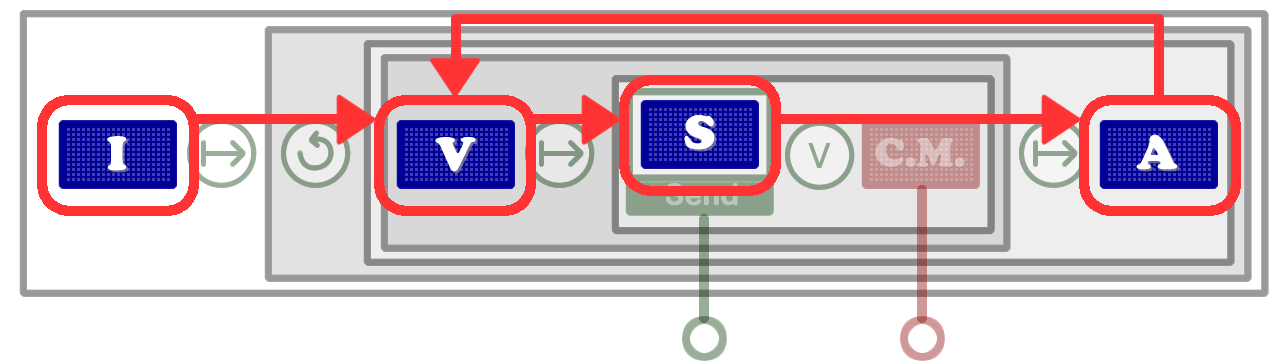
\includegraphics[width=0.7\linewidth]{muta1_v1.png} %[width=0.2\textwidth]{muta1}
}\\
%\hspace{0.05\textwidth}%
\subfloat[][The solver uses the information coming from an external solver]{%
	\label{subfig:beh2}
	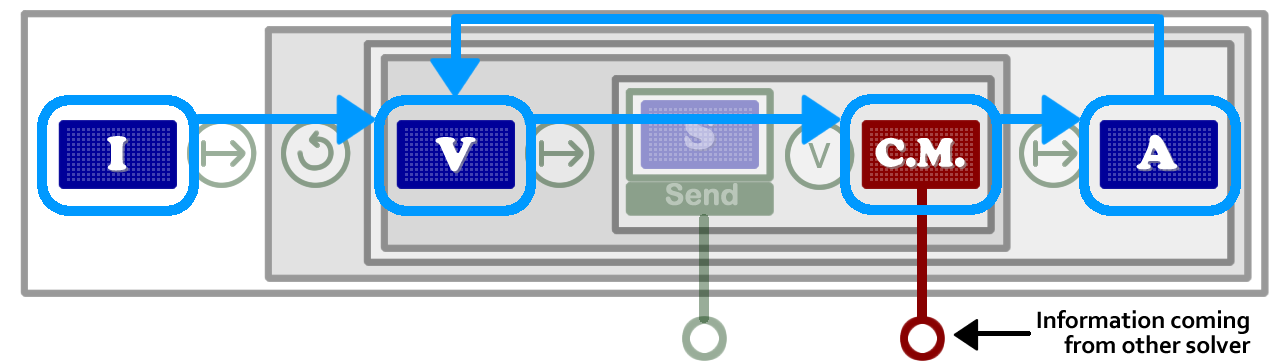
\includegraphics[width=0.7\linewidth]{muta2_v1.png}%[width=0.2\textwidth]{muta2}
}
\caption[]{Two different behaviors in the same solver}
\label{fig:2difBeh}
\end{figure}

In the following Definitions, the concepts of {\it cooperative parallelism} and {\it competitive parallelism} are implicitly included. We say that cooperative parallelism exists when two or more processes are running separately, they are independent, and the general result will be some combination of the results of all the involved processes (e.g. Definitions~\ref{op:min} and~\ref{op:max}). On the other hand, competitive parallelism arise when the general result is the solution of the first process terminates (e.g. Definition~\ref{op:race}).

\begin{definition}\label{op:min}
{\bf (Operator Minimum)} Let the modules
\begin{enumerate}%\begin{inparaenum}[i)]
	\item $\mathcal{M}_1 : \mathcal{D}_1 \rightarrow \mathcal{I}_1$ and  
	\item $\mathcal{M}_2 : \mathcal{D}_2 \rightarrow \mathcal{I}_2$,
\end{enumerate}%\end{inparaenum} 
be, where $\mathcal{D}_1 \subset \mathcal{D}_2$ and $\mathcal{I}_1 \subset \mathcal{I}_2$. Let also $o_1$ and $o_2$ be the outputs of $\mathcal{M}_1$ and $\mathcal{M}_2$ respectively, and assume that there exist some order criteria between them. Then, the operation $\left|\mathcal{M}_1\circled{m}\mathcal{M}_2\right|$ defines the \cm{} $\mathcal{M}_{min}$ that executes $\mathcal{M}_1$ and returns $\min\left\{o_1,o_2\right\}$:

\[
\mathcal{M}_{min}:\mathcal{D}_1\cap\mathcal{D}_2 \rightarrow \mathcal{I}_1 \cup \mathcal{I}_2 
\]
\end{definition}

Similarly we define the operator \textbf{Maximum}:

\begin{definition}\label{op:max}
{\bf (Operator Maximum)} Let the modules
\begin{enumerate}%\begin{inparaenum}[i)]
	\item $\mathcal{M}_1 : \mathcal{D}_1 \rightarrow \mathcal{I}_1$ and  
	\item $\mathcal{M}_2 : \mathcal{D}_2 \rightarrow \mathcal{I}_2$,
\end{enumerate}%\end{inparaenum} 
be, where $\mathcal{D}_1 \subset \mathcal{D}_2$ and $\mathcal{I}_1 \subset \mathcal{I}_2$. Let also $o_1$ and $o_2$ be the outputs of $\mathcal{M}_1$ and $\mathcal{M}_2$ respectively, and assume that there exist some order criteria between them. Then, the operation $\left|\mathcal{M}_1\circled{M}\mathcal{M}_2\right|$ defines the \cm{} $\mathcal{M}_{max}$ that executes $\mathcal{M}_1$ and returns $\max\left\{o_1,o_2\right\}$:

\[
\mathcal{M}_{max}:\mathcal{D}_1\cap\mathcal{D}_2 \rightarrow \mathcal{I}_1 \cup \mathcal{I}_2 
\]
\end{definition}

\begin{definition}\label{op:race}
{\bf (Operator Race)} Let the modules
\begin{enumerate}%\begin{inparaenum}[i)]
	\item $\mathcal{M}_1 : \mathcal{D}_1 \rightarrow \mathcal{I}_1$ and  
	\item $\mathcal{M}_2 : \mathcal{D}_2 \rightarrow \mathcal{I}_2$,
\end{enumerate}%\end{inparaenum} 
be, where $\mathcal{D}_1 \subset \mathcal{D}_2$ and $\mathcal{I}_1 \subset \mathcal{I}_2$. Then, the operation $\left|\mathcal{M}_1\circled{$\shortdownarrow$}\mathcal{M}_2\right|$ defines the \cm{} $\mathcal{M}_{race}$ that executes both modules $\mathcal{M}_1$ and $\mathcal{M}_2$, and returns the output of the module ending first:

\[
\mathcal{M}_{race}:\mathcal{D}_1\cap\mathcal{D}_2 \rightarrow \mathcal{I}_1 \cup \mathcal{I}_2 
\]
\end{definition}

%
%\figalgosbs{
%	\includegraphics[width=\textwidth]{Ex2.eps}
%	\caption{}\label{fig:ex2}
%}{
%\caption{POSL code for Figure \ref{fig:ex2}}
%\dontprintsemicolon
%\SetNoline	
%	$\mathcal{M}_1 \longmapsto \left[\left[\mathcal{M}_4 \circled{$\shortdownarrow$} \mathcal{M}_5\right]\circled{$\times$}\left[\mathcal{M}_2\longmapsto\mathcal{M}_3\right]\right]$\; 
%	$\longmapsto\mathcal{M}_6$\;			
%\label{algo:ex2}
%}
%
%%\begin{example}
%%Suppose that we have the following \module s for selecting a configuration from a defined set (neighborhood): {\sc SelectRandom} selects a random configuration $S^*$ from $\mathcal{V}(S)$, and {\sc SelectBest} selects the $S^*=\argmax\left\{f\left(S_i\right)\right\}, \forall S_i \in\mathcal{V}(S)$. Then, we can define a \module $\mathcal{M}$ that selects the best configuration in the neighborhood, but sometimes it takes a random one:
%%\mybox{
%%	$\mathcal{M}_1 \leftarrow$ {\sc SelectRandom}\\
%%	$\mathcal{M}_2 \leftarrow$ {\sc SelectBest}\\
%%	$\mathcal{M} \leftarrow \mathcal{M}_1\circled{$\rho$}\mathcal{M}_2$ 
%%}
%%\end{example}


The operators presented in Definitions~\ref{op:min}, \ref{op:max} and~\ref{op:race} are very useful in terms of sharing not only information between solvers, but also {\it behaviors}. If one of the operands is a \opch{} it can receive an external solver's \om{}, providing the opportunity to instantiate it in the current solver. The operator either instantiates that module if it is not null, and executes it; or it executes the other operand module otherwise.

Some others operators can be useful dealing with {\it sets}.

\begin{definition}\label{op:union}
{\bf (Operator Union)} Let the modules
\begin{enumerate}%\begin{inparaenum}[i)]
	\item $\mathcal{M}_1 : \mathcal{D}_1 \rightarrow \mathcal{I}_1$ and  
	\item $\mathcal{M}_2 : \mathcal{D}_2 \rightarrow \mathcal{I}_2$,
\end{enumerate}%\end{inparaenum} 
be, where $\mathcal{D}_1 \subset \mathcal{D}_2$ and $\mathcal{I}_1 \subset \mathcal{I}_2$. Let also $V_1$ and $V_2$ be the outputs of $\mathcal{M}_1$ and $\mathcal{M}_2$ respectively. Then, the operation $\left|\mathcal{M}_1\circled{$\cup$}\mathcal{M}_2\right|$ defines the \cm{} $\mathcal{M}_{\cup}$ that executes both modules $\mathcal{M}_1$ and $\mathcal{M}_2$, and returns $V_1\cup V_2$:

\[
\mathcal{M}_{\cup}:\mathcal{D}_1\cap\mathcal{D}_2 \rightarrow \mathcal{I}_1 \cup \mathcal{I}_2
\]
\end{definition}

Similarly we define the operators \textbf{Intersection} and \textbf{Subtraction}:

\begin{definition}\label{op:intersec}
{\bf (Operator Intersection)} Let the modules
\begin{enumerate}%\begin{inparaenum}[i)]
	\item $\mathcal{M}_1 : \mathcal{D}_1 \rightarrow \mathcal{I}_1$ and  
	\item $\mathcal{M}_2 : \mathcal{D}_2 \rightarrow \mathcal{I}_2$,
\end{enumerate}%\end{inparaenum} 
be, where $\mathcal{D}_1 \subset \mathcal{D}_2$ and $\mathcal{I}_1 \subset \mathcal{I}_2$. Let also $V_1$ and $V_2$ be the outputs of $\mathcal{M}_1$ and $\mathcal{M}_2$ respectively. Then, the operation $\left|\mathcal{M}_1\circled{$\cap$}\mathcal{M}_2\right|$ defines the \cm{} $\mathcal{M}_{\cap}$ that executes both modules $\mathcal{M}_1$ and $\mathcal{M}_2$, and returns $V_1\cap V_2$:

\[
\mathcal{M}_{\cap}:\mathcal{D}_1\cap\mathcal{D}_2 \rightarrow \mathcal{I}_1 \cup \mathcal{I}_2
\]
\end{definition}

\begin{definition}\label{op:subst}
{\bf (Operator Subtraction)} Let the modules
\begin{enumerate}%\begin{inparaenum}[i)]
	\item $\mathcal{M}_1 : \mathcal{D}_1 \rightarrow \mathcal{I}_1$ and  
	\item $\mathcal{M}_2 : \mathcal{D}_2 \rightarrow \mathcal{I}_2$,
\end{enumerate}%\end{inparaenum} 
be, where $\mathcal{D}_1 \subset \mathcal{D}_2$ and $\mathcal{I}_1 \subset \mathcal{I}_2$. Let also $V_1$ and $V_2$ be the outputs of $\mathcal{M}_1$ and $\mathcal{M}_2$ respectively. Then, the operation $\left|\mathcal{M}_1\circled{-}\mathcal{M}_2\right|$ defines the \cm{} $\mathcal{M}_{-}$ that executes both modules $\mathcal{M}_1$ and $\mathcal{M}_2$, and returns $V_1 - V_2$:

\[
\mathcal{M}_{-}:\mathcal{D}_1\cap\mathcal{D}_2 \rightarrow \mathcal{I}_1 \cup \mathcal{I}_2
\]
\end{definition}

Now, we define the operators that allow us to send information to outside, i.e. other solvers. We can send two types of information: 
\begin{inparaenum}[i)]
	\item we can execute the \om{} and send its output, or 
	\item we can send the \om{} itself.
\end{inparaenum}. This utility is very useful in terms of sharing behaviors between solvers.

\begin{definition}\label{op:osend}
{\bf (Operator Send Data)} Let the module $\mathcal{M} : \mathcal{D} \rightarrow \mathcal{I}$ be. Then, the operation $\left|\llparenthesis \mathcal{M}\rrparenthesis^{o}\right|$ defines the \cm{} $\mathcal{M}_{sendD}$ that executes the module $\mathcal{M}$ then return and sends its output to outside:

\[
\mathcal{M}_{sendD}:\mathcal{D} \rightarrow \mathcal{I}
\]
\end{definition}

Similarly we define the operator \textbf{Send Module}:

\begin{definition}\label{op:msend}
{\bf (Operator Send Data)} Let the module $\mathcal{M} : \mathcal{D} \rightarrow \mathcal{I}$ be. Then, the operation $\left|\llparenthesis \mathcal{M}\rrparenthesis^{m}\right|$ defines the \cm{} $\mathcal{M}_{sendM}$ that executes the module $\mathcal{M}$, then returns its output and sends the module itself to outside:

\[
\mathcal{M}_{sendM}:\mathcal{D} \rightarrow \mathcal{I}
\]
\end{definition}


Once all desired abstract modules are linked together with operators, we obtain what we call an \as. To implement a concrete solver from an \as, one must instantiate each abstract module with a concrete one respecting the required signature. From the same \as, one can implement many different concrete solvers simply by instantiating abstract modules with different concrete modules.

An \as{} is defined as follow: after declaring an \mbox{\tet{\bf abstract solver}} and its name, the first line defines the list of signatures of \oms, the second one the list of signatures of \opchs, then the algorithm of the solver is defined is the solver's body, between \mbox{\tet{\bf begin}} and \mbox{\tet{\bf end}}. For instance, Algorithm~\ref{algo:as_example} illustrate the abstract solver corresponding to Figure~\ref{subfig:as}.


\begin{algorithm}[H]
\caption{\posl{} code for solver presented in Figure~\ref{subfig:as}}
		\dontprintsemicolon
		\SetNoline
		\SetKwProg{myproc}{}{}{}
		\myproc{\tet{\bf abstract solver} solver\_01\;
		\tet{\bf computation} : $I, V, S, A$ \; 
		\tet{\bf connection}: $C.M.$}{
			\Begin{
				%\While{$($\Iter $< K_1)$}
				%{
					$I$ \sec \; %\circled{$\mapsto$}$\;
					\While{$($\Iter \% $K_2)$}{
						$V$ \sec $\left[C.M.\textbf{  } \circled{$\vee$} \textbf{  } \llparenthesis S\rrparenthesis^o\right]$ \sec $A$\;
					}
				%}
			}
		}
		\label{algo:as_example}
\end{algorithm}	

\section{Third Stage: Creating \posl{} solvers}

With operation modules and open channels already assembled through the \as, we can create solvers by instantiating modules. \posl{} provides an environment to this end and we present the procedure to use it. 

\section{Forth Stage: Connecting the solvers}

Once we have defined our solver strategy, the last step is to declare the \comstrs, i.e. connecting the solvers each others. In this last stage, \posl{} provides to the user a platform to easily define cooperative meta--strategies that solvers must follow (\posl{} meta--solvers). The steps to create \comstrs{} through \textit{communication operators} are explained and some examples are presented. We explain how to create new \textit{communication operators} using the basic layer of the framework.

\section{Fifth Stage: Modeling the target benchmark}

In this stage we explain formally our modeling process of a benchmark to be solved (or study) through \posl{}. We explain how to make use of the already existing models or to create new benchmarks using the basic layer of the framework in C++ making a proper usage of the object-oriented design.

\section{Step-by-step \posl{} code example}

In this section we summarize all the steps to build a \posl{} meta--solver through an real example, providing schemes to make more comprehensive the process.
